\chapter{Active Debugging and Applications of Live Debugging}
\label{ch:activedebugging}

\section{Overview}
\label{sec:guided_overview}

In the sections uptil now, we have introduced a framework for \livedebugging, a tool for pre-packaging binaries to make them \livedebugging friendly. 
We now discuss some applications of \livedebugging in the real-world, and in particular introduce a new mechanism called \activedebugging.


The debug container allows for debuggers to apply any ad-hoc technique used in offline debugging.
However, in order for us to have continuous debugging, it is essential to allow for forward progress in the debug container. 
Furthermore, the divergence due to instrumentation (either due to slowdown, or functional) should not stop forward-progress in the debug-container.
Having a debug-container which is isolated from the production, but still in sync with production services, allows a variety of ad-hoc debugging approaches to be integrated and leverage our framework.
Traditional offline debugging approaches, such as dynamic instrumentation can be easily directly applied to the debug-container without any ramifications. 
Others like memory or performance profiling, and execution traces can also be applied in the debug container.
Similarly the \debugcontainer can be used as a staging mechanism for record-replay on demand to ensure deterministic execution.
The key to applying these approaches is that none of them functionally modifies the application.

This chapter is divided in the following key parts: Firstly, in section~\ref{sec:guidedDiscussion}, we discuss the advantages and limitations of \parikshan in real-world settings.
Furthermore, we highlight certain key points that the debugger most be aware of when debugging applications with \parikshan, so that he can do reliable and fast debugging. 
In section~\ref{sec:activeDebuggingScenarios}, we classify debugging production applications in two high level debugging scenario categories: \emph{post-facto}, and \emph{proactive} analysis.
We leverage these classifications to explain how different techniques can be applied in \parikshan, and in which scenarios debugging on the fly does not make sense.
Next we list some existing debugging technologies, like statistical debugging, execution tracing, record and replay etc. to explain how they can be either directly applied or modified slightly and applied with the \parikshan framework to significantly improve their analysis.

In the next section, we introduce \activedebugging whereby developers can apply a patch/fix or apply a test in the \debugcontainer.
\activedebugging ensures that any modifications in the \debugcontainer does not lead to a state change in the \productioncontainer.
This will enable the debugger to fix/patch or run test-cases in the debug-container while ensuring forward progress and in sync with production. 
We are inspired from existing perpetual invivo testing frameworks like INVITE~\cite{invivo}(which also provides partial test-isolation), in the production environment.
We currently restrict \active debugging to patches/and test-cases only bring about local changes, and not global changes in the application.

In the last section we introduce budget-limited adaptive instrumentation. Which focuses further on how to allow for continuous debugging with the maximum information gain.
One of the key criteria for successful statistical debugging is to have higher instrumentation rates, to make the results more statistically significant. 
There is a clear trade-off between instrumentation vs performance overhead for statistical instrumentation. 
A key advantage of using this with \parikshan is that we can provide live feedback based buffer size and bounded overheads, hence squeezing the maximum advantage out of statistical debugging without impacting the overhead. 
We evaluate the slack available in each request for instrumentation without risking a buffer overflow and getting out of sync of the production container.
Live interactive debugging provided by \parikshan further allows for quick updates to the instrumentation and targeting specific areas of the application code.
Budget limited instrumentation is inspired from statistical debugging~\cite{statisticalDebugging}, and focuses on a two-pronged goal of bounding the instrumentation overhead to avoid buffer overflows in \parikshan, and simulatneously have maximum feedback regarding information gained from real-time instrumentation.

\xxx{This section is divided in the 3 parts: First in section, next in section, next in section, }

\iffalse
One possible route that we wish to explore further is how to allow for validation of test-cases, or validate functional patches/fixes, which may modify the output.
For the purposes of our exploration, we have currently assumed that these patches/and test-cases only bring about local changes, and not global changes in the application.
In this section, we introduce the concept of \activedebugging, whereby developers can apply a patch/fix or apply a test in the \debugcontainer.
\activedebugging ensures that any modifications in the \debugcontainer does not lead to a state change in the \productioncontainer.
This will enable the debugger to fix/patch or run test-cases in the debug-container while ensuring forward progress and in sync with production. 
We are inspired from existing perpetual invivo testing frameworks like INVITE~\cite{invivo}(which also provides partial test-isolation), in the production environment.

In recent years several monitoring techniques have been developed to monitor the health of production systems.
For example most modern operating systems have resource monitors~\cite{linuxHealth, windowsHealth, macHealth}, which can be used to track the CPU, memory usage, cache misses, temperature etc. of the physical machine.
These are useful to discover high workloads, or if the machine is stressed because of heavy resource usage.
Similarly, application level monitoring tools are used to report transactions or errors in the application.
Monitoring outputs usually provide the first clue towards resolving an error in the debugging process.
%While useful, these monitoring mechanisms  have a performance trade-off with the amount of instrumentation that can be done.
%Furthermore, the information provided by these logs may not be enough to understand the root-cause of the error.

However all monitoring/instrumentation techniques impose a performance overhead on the applications.
This can adversely impact user-experience, hence real-world production instrumentation is generally kept at very low levels.
\parikshan provides an alternative mechanism where this debugging/instrumentation can be done in parallel on a sandboxed cloned container.
Any instrumentation or monitoring in the debug-container has no performance impact on the production container.
In the context of our system, debuggers can use a variety of ad-hoc approaches to capture the root-cause of an error.
For example a naive approach could be to use trial-and-error instrumentation to find the execution trace for the error.
Alternatively, the user could also do aggressive brute force instrumentation for all function execution, which could help locate the problem.
However, both these approaches can have potentially high overheads, which in turn can lead to a buffer overflow.

In this chapter we introduce a statistical sampling approach which imposes a bounded performance overhead, to ensure maximal live debugging information, without causing a buffer overflow.
%In our search for more systematic approach towards live debugging, we looked towards two possible techniques.
%Firstly, we try to implement an automated budget limited instrumentation approach for capturing application logs.
We are inspired by previous work done in statistical debugging~\cite{cbi}, and delta debugging~\cite{delta} techniques which aim to streamline and automate the process of bug localization.
This is achieved by having predicate profiles from both successful and failing runs of a program and applying statistical techniques to pinpoint the cause of the failure.
The core advantage of statistical debugging is that the sampling frequency of the instrumentation can be decreased to reduce the instrumentation overhead.

One of the key criteria for successful statistical debugging is to have higher instrumentation rates, to make the results more statistically significant. 
There is a clear trade-off between instrumentation vs performance overhead for statistical instrumentation. 
A key advantage of using this with \parikshan is that we can provide live feedback based buffer size and bounded overheads, hence squeezing the maximum advantage out of statistical debugging without impacting the overhead. 
We evaluate the slack available in each request for instrumentation without risking a buffer overflow and getting out of sync of the production container.
Live interactive debugging provided by \parikshan further allows for quick updates to the instrumentation and targeting specific areas of the application code.
\fi

\section{Live Debugging using Parikshan}
\label{sec:guidedDiscussion}

The following are some key advantages of \parikshan that can be leveraged for debugging user-facing applications on the fly:

\begin{itemize}
	
	\item \textbf{Sandboxed Environment}: The debug container runs in a sandboxed environment which is running in parallel to the real production system, but any changes in the \debugcontainer are not reflected to the end-user. This is a key advantage in several debugging techniques which are disruptive, and can change the final output. 
	
	Normal debugging mechanisms such as triggering a breakpoints or patching in a new exception/assertion to figure out if a particular "condition" in the application system state is breaking the code, cannot be done in a production code as it could lead to a critical system crash. On the other hand, \parikshan's debug containers are ideal for this scenario as they will allow developers to put in a patches without any fear of system failure.
	
	\item \textbf{Zero Overhead Monitoring}:The most novel aspect of \parikshan is that it allows for zero overhead monitoring of the production system. This means that high-overhead debugging techniques can be applied on the debug-container without incurring a slow-down in production.
	
	Debugging techniques like record-replay tools which have traditionally high recording overheads can generally not be applied in production systems. However, \parikshan can be used to decouple the recording overhead from production, and can allow for relatively higher overhead recording with more granularity.
	
	\item \textbf{Capturing production system state}:
	One of the key factors behind capturing the root-cause of any bug is to capture the system state in which it was triggered. \parikshan has a live-cloning facility that clones the system state and creates a replica of the production. Assuming that the bug was triggered in the production, the replica captures the same state as the production container.
	
	\item \textbf{Compartmentalizing large-scale systems context}:
	Most real-world services are deployed using a combination of several SOA applications, each of them interacting together to provide an end-to-end service. This could be a traditional 3 tier commerce system, with an application layer, a database layer and a web front-end, or a more scaled out social media system with compute services, recommendation engines, short term queuing systems as well as storage and database layers. 
	Bugs in such distributed systems are particularly difficult to re-create as they require the entire large-scale system to be re-created in order to trigger the bug. 
	Traditional record-replay systems if used are insufficient as they are usually focused on a small subset of applications.
	
	Since, our framework leverages network duplication, \parikshan can allow looking at applications in isolation and capturing the system state as well as the input of the running application, without having to re-create the entire buggy infrastructure. 
	In a complex multi-tier system this is a very useful advantage to localize the bug.
	
	
\end{itemize}

At the same time there are some things that the administrator must be aware of

\begin{itemize}
	\item \textbf{Continuous Debugging and Forward Progress}:
	\livedebugging allows users to debug applications on-the-fly. The debug-container where one can do debugging runs in parallel to the production container. This is done by first making a live replica of the system followed by duplicating and sending the network input to the \debugcontainer. 
	In a way the \debugcontainer still communicates with the entire system although it's responses are dropped. 
	To ensure forward progress in the \debugcontainer, it is essential that the \debugcontainer is in-sync with the production container, so that the responses, and the requests from the network are the expected responses for forward progress in the application running on the \debugcontainer.
	
	Take for instance, a MySQL~\cite{mysql} service running in the \productioncontainer and \debugcontainer. If during our debugging efforts we modify the state of the debug service such that the MySQL database is no longer in synch with the production service, then any future communication from the network could lead to the state of the debug-container to further diverge from the production. Additionally, depending on the incoming requests or responses the debug application may crash or not have any forward progress.
	
	No forward-progress does not necessarily mean that debugging cannot take place, however for continuous debugging to take place, once the machine has crashed it needs to be re-cloned from the production container, for further debugging. Further, given programmer knowledge the debugger can try his best to avoid state changes that would lead to an un-intentional crash.
	
	\item \textbf{Debug Window}:
	As explained earlier, most debugging mechanisms generally requires instrumentation and tracking execution flow. This means that the application will spend some compute cycles in logging instrumentation points thereby having a slow-down. While \parikshan avoids any slow-down in the production environment, there will be some slow-down in the debug-container. 
	
	The amount of time till which the production container remains in synch with the \debugcontainer is called the debug-window(see section~\ref{sec:window}). The window time depends on the overhead, the size of the buffer and the incoming request rate. If a buffer overflow happens because the debug-window has finished, the \debugcontainer needs to be re-synced with the production container.
	
	In our experiments, we have observed, that \parikshan is able to accomodate significant overhead without incurring a buffer overflow.	
	Administrators or debuggers using \parikshan should keep the overhead of their instrumentation in mind when debugging in \parikshan. Ofcourse they can always re-clone the \productioncontainer to start a new debugging session.
	
	\item \textbf{Non-determinism}:
	
	One of the most difficult bugs to localize are non-deterministic bugs. While \parikshan is able to capture system non-determinism by capturing the input, it is unable to capture thread non-determinism. Most service-oriented applications have a large number of threads/processes, which means that different threading schedules can happen in the production container as compared to the debug-container.
	This means, that a specific ordering of events that caused a bug to be triggered in the production container, may not happen in the debug-container.
	
	There are multiple ways that this problem can be looked at. Firstly, while it's difficult to quantify, for all the non-deterministic cases in our case-studies, we were able to trigger the bug in both the production and the replica. 
	In the case where the bug is actually triggered in the \debugcontainer, the debugging can take place as usual for other other bugs.
	If that is not the case, there are several techniques which provide systematic "search" for different threading schedules based on a high granularity recording of all potential thread synchronization points, and read/write threads. While such high granularity recording is not possible in the production container, it can definitely be done in the \debugcontainer without any impact on the production service.
	
\end{itemize}

\section{Debugging Scenarios}
\label{sec:activeDebuggingScenarios}

Based on our casestudies, and survey of commonly seen SOA bugs we classify the following scenarios for live debugging. 
In each of the scenarios we explain how different categories of bugs can be caught or analyzed.

\subsection{Scenario 1: Post-Facto Analysis}
\label{sec:activePostFactoAnalysis}

In this scenario, the error/fault happens without \livedebugging having been turned on i.e. the service is only running in the production container, and there is no replica.
Typically light-weight instrumentation or monitoring is always turned on in all service/transaction systems. 
Such monitoring systems are very limited in their capabilities to localize the bug, but they can indicate if the system is in a faulty state.

For our post-facto analysis, we use such monitoring systems as a trigger to start \livedebugging once faulty behvaior is detected. 
The advantage of such an approach is that debugging resources are only used on-demand, and in an otherwise normal system only the \productioncontainer is utilizing the resources.


There are three kind of bugs that can be considered in this kind of situation:

\begin{itemize}
	
	\item \textbf{Persistent Stateless Bugs}: 
	
	This is the ideal scenario for \parikshan.
	Persistent bugs are those that persist in the application and are long running. 
	They can impact either some or all the requests in a SOA application.
	Common examples of such bugs are memory leak, performance slow-down, semantic bugs among others.
	Assuming they are statistically significant, persistent bugs will be triggered again and again by different requests.
	
	We define \emph{stateless bugs} here as bugs which do not impact the state of the system, hence not impacting future queries. 
	For instance read only operations in the database are stateless, however a write operation which corrupts or modifies the database is stateful, and is likely to impact and cause errors in future transactions.
	
	Hence, such bugs are only dependent on the current system state, and the incoming network input.
	Once such a bug is detected in the production system, \parikshan can initiate a live cloning process and create a replica for debugging purposes. 
	Assuming similar inputs which can trigger the bug are sent by the user, the bug can be observed and debugged the \debugcontainer.
	
	\item \textbf{Persistent Stateful Bugs}:
	
	Stateful bugs are those bugs which can impact the state and change it such that any such bug impacts future transactions in the production container as well.
	For instance in a database service a table may have been corrupted, or it's state changed so that certain transactions are permanently impacted. 
	While having the execution trace of the initial request which triggered a faulty state is useful, the ability to analyze the current state of the application is also extremely useful in localizing the error.
	
	Creating a live clone after such an error and checking the responses state of future impacted transaction, as well as the current state of the database can be a good starting point towards resolving the error. 
	
	\item \textbf{Crashing Bugs}: 
	
	Crashing bugs are bugs that lead to a crash in the system thereby stopping the service.
	Unhandled exceptions, or system traps are generally the cause of such crashes.
	Unfortunately \parikshan has limited utilization for post-facto analysis of a crashing bug. 
	Since \parikshan is not turned "on" at the time of the crash, any post-facto analysis for creating a \debugcontainer is not possible.

	
\end{itemize} 

\subsection{Scenario 2: Proactive Analysis}
\label{sec:activeProactiveAnalysis}

Proactive analysis are scenarios where the user starts debugging when the system is performing normally and their is no bug. This is the same as having instrumentation on or monitoring a production server, except that in this case the instrumentation is actually present in the \debugcontainer.

One possible scenario is to use the \debugcontainer to do recording or high granularity instrumentation. This is extremely useful feature to have if you expect to have higher overheads of instrumentation, which are unacceptable in the production environment. 
On the other hand our \debugcontainer can have much higher instrumentation without any performance penalty on the production container.
Another useful feature of staged recording is the case where the debugger needs to put in breakpoints or potentially instrumentation which can cause the system to crash can also be put in the \debugcontainer
Proactive recording is basically use to track bugs that could happen in the future as the transaction or request which causes the failure is caught as well, as well as it is caught in the context of the system state. 
Once a bug is caught, the cause can be independently explored in the \debugcontainer.

Proactive Analysis, is useful for both stateless and stateful bugs, we do not differentiate between them here as even in the case of a stateful bug, debugging is always turned on. 
Proactive approaches can be compared to existing approaches like statistical debugging~\cite{statisticalDebugging} which use active statistical profiling to compare between successful and buggy runs, to isolate the problem. We discuss statistical debugging in section~\ref{sec:activeStatisticalDebugging} and present an advanced approach in section~\ref{sec:activeBudgetLimited}.
Other proactive body of work include record-replay infrastructures, which record production systems, and can replay the execution if a bug is discovered.
In section~\ref{sec:activeStagedRecordReplay}, we have discussed staged record-and-replay, which is an advanced record-replay technique that can be applied with the help of \parikshan.



\section{Existing Debugging Mechanisms}
\label{sec:activeExistingTechniques}

\subsection{Execution Tracing}
\label{sec:activeExecutionTracing}

One of the most common techniques to debug any application is execution tracing. 
Execution tracing gives a trace log of all the functions/modules executed when an input is received. 
This helps the debugger in looking at only those execution points and makes it easier to reason out what is going wrong.

Execution tracing can happen at different granularities: for instance an application can be monitored at function level granularity (only entry and exit of function is monitored), or for deeper understanding at read/write, synchronization point or even instruction level granularity.
Depending on how much granularity the tracing is done at the overhead may be unacceptable for production systems.

Execution tracing can be de-coupled from original execution and put in \debugcontainer for higher granularity instrumentation. 
Such techniques which decouple execution and analysis also been previously explored in papers like Aftersight~\cite{aftersight} and DoublePlay~\cite{doubleplay}.
\parikshan provides a systematic framework for decoupling without enforcing strong constraints on the user.

\subsection{Statistical Debugging}
\label{sec:activeStatisticalDebugging}

Statistical debugging aims to automate the process of isolating bugs by profiling several runs of the program and using statistical analysis to pinpoint the likely causes of failure. 
The seminal paper on statistical debugging~\cite{statisticalDebugging}, has lead to several advanced approaches~\cite{holmes,adaptive,statisticalPerformance}, and is now a well established debugging methedology. 

The core mechanism of statistical debugging is to have probabilistic profiling, by sampling execution points and comparing the execution traces for failed and successful transactions.
It then uses statistical models to identify path profiles that are strongly predictive of failure. 
This can be used to iteratively localize the bug causing execution, and can then be manually analyzed by \parikshan.

Statistical debugging is one of the systematic bug localization approaches that can be directly applied in the \debugcontainer, with the added advantage that the amount of instrumentation that can be applied in the debug-container is much higher than production containers. 
Apart from regular semantic bugs, previous body of works have shown that statistical debugging is useful in detecting a variety of other bugs like concurrency bugs~\cite{statisticalConcurrency}, and performance~\cite{statisticalPerformance}.

\subsection{Staging Record and Replay}
\label{sec:activeStagedRecordReplay}

\begin{figure}[h!]
	
	\centering
	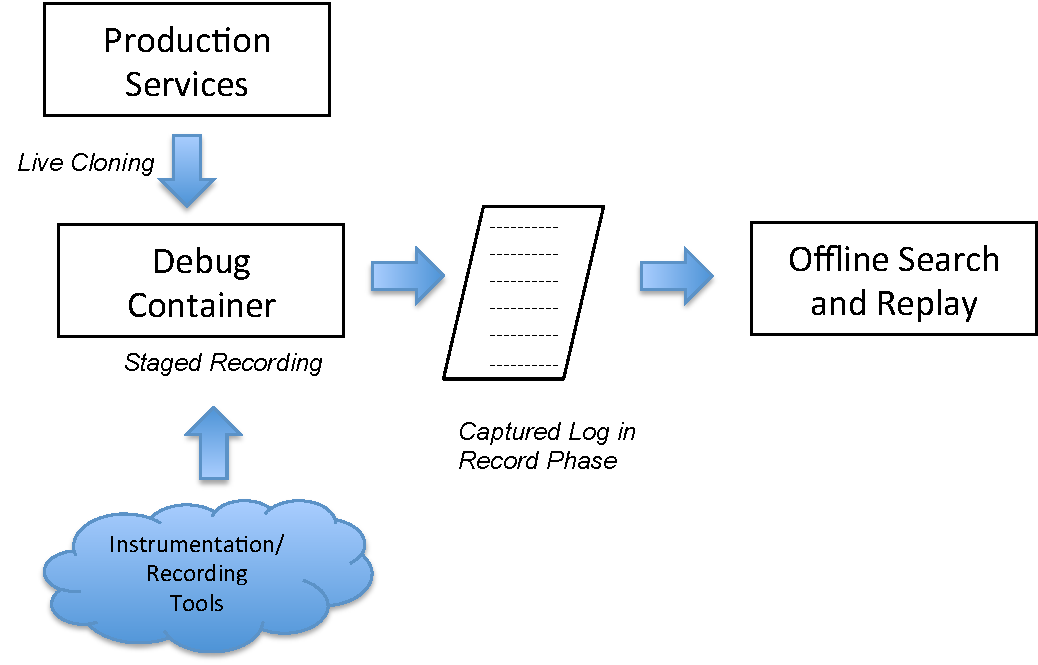
\includegraphics[width=0.99\textwidth]{guided/figs/stagedRecordReplay.pdf}
	\caption{Staged Record and Replay using \parikshan}
	\label{fig:stagedRecordReplay}
\end{figure}

One well known sub-category of debugging service-oriented applications are record-replay infrastructures.
In the past decade there have been numerous record-and-replay infrastructures which have been introduced in academia.
The core focus of these techniques is to faithfully reproduce the execution trace and allow for offline debugging.
However, in order faithfully reproduce the exact same instrumentation, the recording phase must record a higher granularity of execution.
Unfortunately, this means a higher overhead at the time of recording in the production system.
Such recording overhead is usually unacceptable in most production systems.

Record and replay can be coupled with the \debugcontainer to avoid any overhead on the \productioncontainer.
This is done by staging the recording for record-and-replay in the \debugcontainer instead of the production, and then replaying that for offline analysis.
In figure~\ref{fig:stagedRecordReplay} we show how the production system can first be "live-cloned". A copy of the container's image can be stored/retained for future offline replay - this incurs no extra overhead as taking a live snapshot is a part of the live-cloning process. Recording can then be started on the \debugcontainer, and logs collected here can be used to do offline replay.

An important aspect to remember here is that \textbf{non-determinism} can lead to different execution flows (with low probability as the system is a clone of the original) in the \debugcontainer v.s. the \productioncontainer.
Hence simply replaying an execution trace in the \debugcontainer, may not lead to the same execution which triggers the bug.
However several existing record-and-replay techniques offer "search" capabilities to replay and search through all possible concurrent schedules which could have triggered a non-deterministic error.
Hence we propose that the exact executing schedule which triggered a bug, and using the \debugcontainer for recording instead of the \productioncontainer is a viable alternative to traditional record-replay techniques.

\subsection{A-B Testing}

\begin{figure}[h!]
	
	\centering
	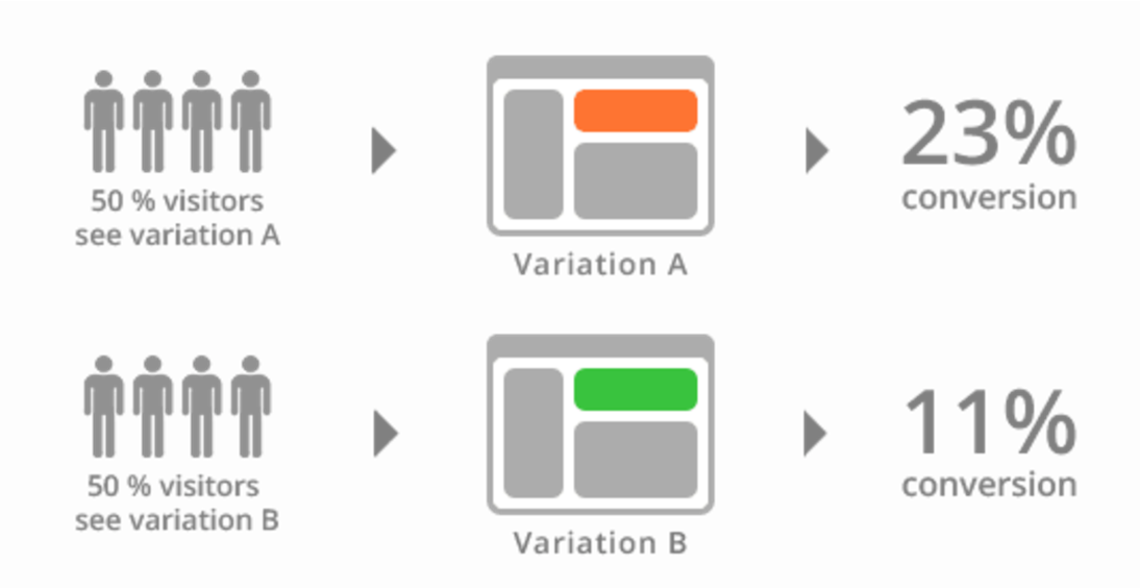
\includegraphics[width=0.99\textwidth]{guided/figs/ABTesting.pdf}
	\caption{Traditional A-B Testing}
	\label{fig:abTesting}
\end{figure}

A/B testing (sometimes called split testing) is comparing two versions of a web page to see which one performs better. 
You compare two web pages by showing the two variants (let's call them A and B) to similar visitors at the same time.
Uer operations in A can then be compared to user scenario's in B to understand which is better, and how well it was received.

Similar A/B Testing, for performance patches or other functional patches, can be done in the \debugcontainer for evaluation of patches which are functionally similar and have same input/output.


\subsection{Interactive Debugging}

The most common debugging tools used in the development environment are interactive debuggers. 
Debugging tools like gdb~\cite{gdb}, pdb, or eclipse~\cite{eclipse}, provide intelligent debugging options for doing interactive debugging. 
This includes adding breakpoints, watchpoints, stack-unrolling etc.
The downside to all of these techniques is that they essentially stop the service or execution.
Once a process has been attached to a debugger, a shadow process in also attached to it and the rest of the execution follows with just-in-time execution, allowing the debugger to monitor the progress step-by-step therefore making it substantially easier to catch the error.
Unfortunately, this cannot be applied to the \productioncontainer.

However this can be easily applied towards the \debugcontainer, where the execution trace can be observed once a breakpoint has been reached.
While this does mean that the replica will not be able to servce any more requests (except for those that have been buffered), the request which is inside the breakpoint will be processed.
Generally breakpoint and step-by-step execution monitoring is used for a limited scope of execution within a single transaction.
Once, finished future transactions can also be debugged after doing a re-sync by applying live cloning again.


\section{Budget Limited, Adaptive Instrumentation}
\label{sec:activeBudgetLimited}

As explained in section~\ref{sec:design}, the asynchronous packet forwarding in our network duplication results in a \debugwindow.
The \debugwindow is the time before the buffer of the debug-container overflows because of the input from the user.
The TCP connection from end-users to production-containers are synchronized by default.
This means that the rate of incoming packets is limited by the amount of packets that can be processed by the production container.
On the other hand, packets are forwarded asynchronously to an internal-buffer in the debug-container.
The duration of the \debugwindow is dependent on the incoming workload, the size of the buffer, and the overhead/slowdown caused due to instrumentation in the debug-container.
Each time the buffer is filled, requests are dropped, and the debug-container can get out of sync with the production container.
To get the debug-container back in sync, the container needs to be re-cloned.
While duplicating the requests has negligible impact on the production container, cloning the production container can incur a small suspend time(workload dependent).
\iffalse
\begin{wrapfigure}{R}{0.75\textwidth}
	\centering
	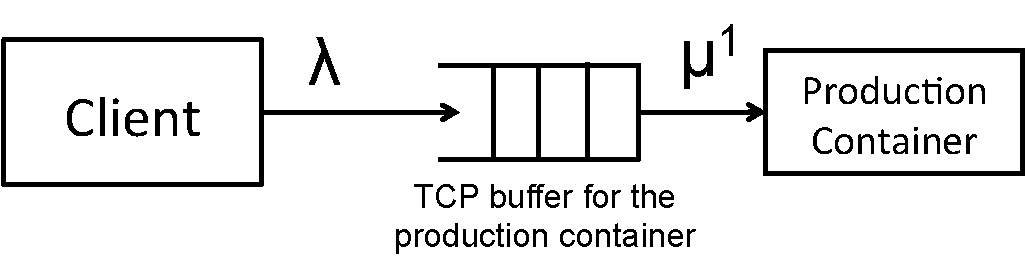
\includegraphics[width=0.45\textwidth]{queue/figs/queue.pdf}
	\caption{\label{fig:queueModel}An example of a simple queue applied to a SOA application. Here the arrival rate of the requests to the queue is a poisson process with rate $\lambda$, and the service time of each request is a poisson process with rate $\mu$. In the default SOA settings, the client request is being sent into a blocking TCP queue, where the incoming requests are rate limited by $\mu$. Hence, there is never any buffer overflow}
\end{wrapfigure}
\fi

The duration of the \debugwindow can be increased by reducing the instrumentation.
At the same time we wish to increase the maximum information that can be gained out of the instrumentation to do an effective bug diagnosis.
Essentially for a given buffer size and workload, there is a trade-off between the information gain due to more instrumentation and the duration of the \debugwindow.
Hence our general objective is to increase the information gain through instrumentation while avoiding a buffer overflow.

We divide this task into  pro-active and re-active approaches which can complement each other. Firstly, we pro-actively assign budgets using queuing theory and simulations. We try to find that assuming a poisson distribution for average processing time of each request and the inter-arrival time of requests, we can find expected buffer sizes for a reasonable debug-window length. Secondly, we propose a re-active mechanism triggered by the amount of buffer used. The buffer utilization can be continuously monitored and the instrumentation sampling can be exponentially reduced if the buffer is near capacity. This can be combined with statistical debugging to have the maximum information gain possible. 

\subsection{Proactive: Modeling Budgets}
\label{sec:activeProactiveModeling}


\begin{figure}[t!]

		\centering
		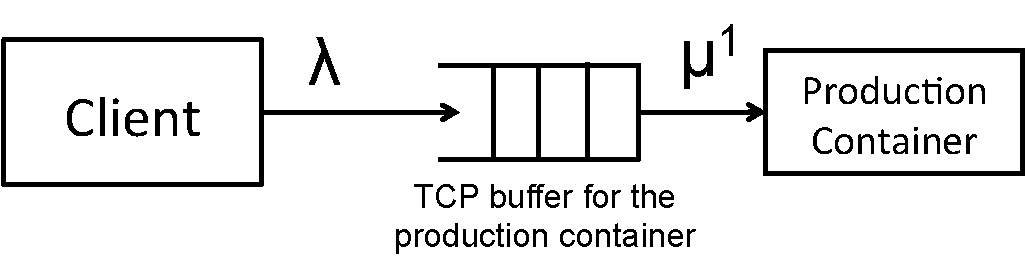
\includegraphics[width=0.99\textwidth]{queue/figs/queue.pdf}
		\caption{\parikshan applied to a mid-tier service}
		\label{fig:queueModel}
\end{figure}
\begin{figure}
		\centering
		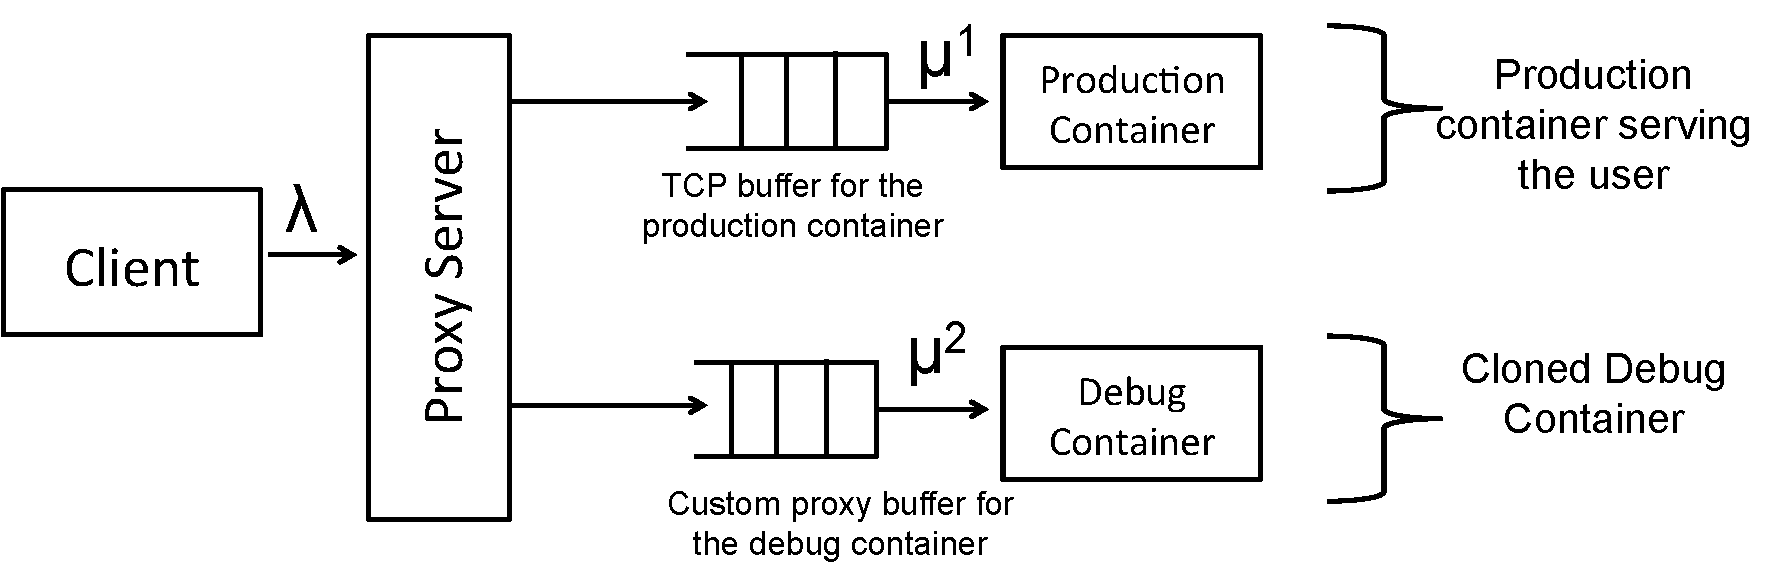
\includegraphics[width=0.99\textwidth]{queue/figs/queueCloned.pdf}
		\caption{External and Internal Mode for live cloning: P1 is the production, and D1 is the debug container.}
		\label{fig:queueClonedModel}
\end{figure}
	
%\caption{Modeling \livedebugging using queuing theory}
%\end{figure*}

\iffalse
\begin{figure}[h]
	\begin{center}
		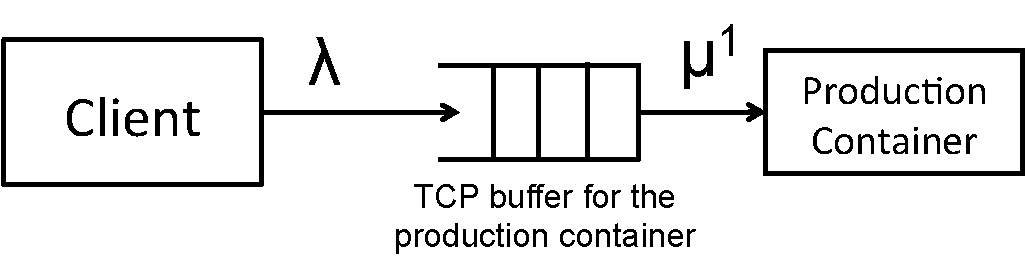
\includegraphics[width=0.8\textwidth]{queue/figs/queue.pdf}
		\caption{An example of a simple queue applied to a SOA application. Here the arrival rate of the requests to the queue is a poisson process with rate $\lambda$, and the service time of each request is a poisson process with rate $\mu$. }
		%\caption{\parikshan applied to a mid-tier service: It is comprised of: (1) Clone Manager for Live Cloning, (2) Proxy Duplicator to duplicate network traffic, and (3) Proxy Aggregator to replay network traffic to the cloned debug container.}
		\label{fig:queueModel}
	\end{center}
\end{figure}
\fi

In this section we try to model the testing window by using concepts well used in queuing theory (for the sake of brevity we will avoid going into too much detail, readers can find more about queuing theory models in~\cite{queueBook}).
Queueing theory is commonly used to do capacity planning for service-oriented architectures(SOA).
Queues in a SOA application can be modeled as a M/M/1/K queue (Kendall's notation~\cite{kendall}).
Kendall's notation is a well known model which allows a compact representation for queues in SOA architectures.
This is a shorthand notation of the type A/B/C/D/E where A, B, C, D, E describe the queue.
%This notation may be easily applied to cover a large number of simple queueing scenarios.
The standard meanings associated with each of these letters are summarized below.\\

\begin{framed}
	\noindent \textbf{A} represents the \emph{inter-arrival time distribution}\\
	\textbf{B} represents the \emph{service time distribution}\\
	\textbf{C} gives the \emph{number of servers} in the queue\\
	\textbf{D} gives the \emph{maximum number of jobs that can be there in the queue}.
	%If this is not given then the default value of infinity \infinity is assumed implying that the queue has an infinite number of waiting positions\\
	\textbf{E} represents the Queueing Discipline that is followed. The typical ones are First Come First Served (FCFS), Last Come First Served (LCFS), Service in Random Order (SIRO) etc. If this is not given then the default queueing discipline of FCFS is assumed.
\end{framed}

\noindent The different possible distributions for \textbf{A} and \textbf{B} above are:

\begin{framed}
	\noindent \textbf{M} exponential distribution\\
	\textbf{D} deterministic distribution\\
	\textbf{E$_{\text{k}}$} Erlangian (order k)\\
	\textbf{G} General
\end{framed}



Figure \ref{fig:queueModel} represents a simple client-server TCP queue in an SOA architecture based on the M/M/1/K queue model.
An M/M/1/K queue, denotes a queue where requests arrive according to a poisson process with rate $\lambda$, that is the inter-arrival times are independent, exponentially distributed random variables with parameter $\lambda$ .
The service times are also assumed to be independent and exponentially distributed with parameter $\mu$. 
Furthermore, all the involved random variables are supposed to be independent of each other.
In the case of a blocking TCP queue common in most client-server models, the incoming request rate from the client is throttled based on the request processing time of the server. 
This ensures that there is no buffer-overflows in the system.

\iffalse
\begin{figure}[h]
	\begin{center}
		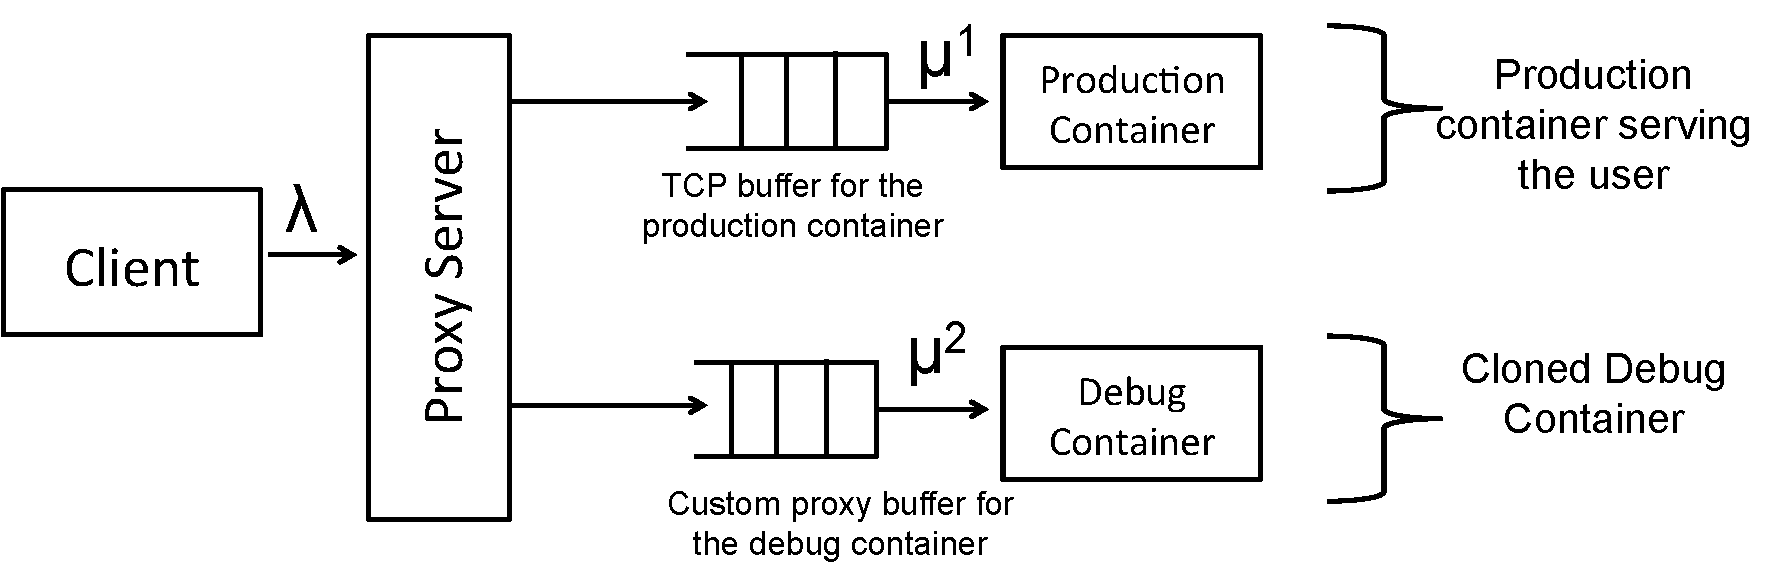
\includegraphics[width=0.8\textwidth]{queue/figs/queueCloned.pdf}
		\caption{This figure shows how the simple queueing model can be extended to \parikshan. Here instead of looking at the TCP buffer, we look at the packet arrival and processing time for the proxy duplicator.}
		%\caption{\parikshan applied to a mid-tier service: It is comprised of: (1) Clone Manager for Live Cloning, (2) Proxy Duplicator to duplicate network traffic, and (3) Proxy Aggregator to replay network traffic to the cloned debug container.}
		\label{fig:queueClonedModel}
	\end{center}
\end{figure}
\fi

In \parikshan, this model can be extended to a cloned model as shown in figure \ref{fig:queueClonedModel}.
The packets to both the production and the debug cloned containers are routed through a proxy which has internal buffer to account for slowdowns in request processing in the debug container. 
Here instead of the TCP buffer, we focus on the request arrival and departure rate to and from the proxy duplicators buffer.
The incoming rate remains the same as $\lambda$, as the requests are asynchronously forwarded to both containers without any slowdown. 
The request processing rate of the debug container is $\mathrm{\mu_{3}}$, where $\mathrm{\mu_{2}}$ $>$ $\mu$ (the processing time for the production container) depending on the overhead due to instrumentation in the debug-container.
To simplify the problem, we assume the outgoing requests from the proxy buffer to be $\mathrm{\mu_{3}}$ where:\\

\begin{equation}
\mu_{3} = \mu_{2} - \mu
\end{equation}

The remaining processing time for both the production container and the debug container is going to be the same. 
Since the TCP buffer in the production container is a blocking queue, we can assume that any buffer overflows in the proxy buffer are only caused because of the instrumentation overhead in the debug-container, which is accounted for by $\mathrm{\mu_{3}}$. 
We borrow from existing theoretical foundation for hitting time, and simulation experiments to find approximate overhead bounds for instrumentation. 
Our model can be further expanded to a load balanced model. Please look at Appendix D for further understanding of these results.

\iffalse
The utilization factor for an M/M/1/K queue can be formulated as follows:

\begin{equation}
\rho = \frac{\lambda}{\mu}
\end{equation}
\\ \\

Now based on this notation and the expected number of requests buffered in the queue the blocking probability for the queue can be calculated as follows:

\begin{equation}
P_{b} = \frac{(1-\rho)\rho^{K}}{1-\rho^{K+1}}
\end{equation}
\\ \\

The expected time for the queue to fill up:

\begin{equation}
E[] =
\end{equation}

Given the expected time for processing each request in this model

\begin{equation}
E[] =
\end{equation}

The overhead bounds for instrumentation in each request can be modeled as follows:

\begin{equation}
E[] = 
\end{equation}

This gives us the following relationship between overhead and expected time for the queue to fill up.

\begin{equation}
E[] = relationship\ with\ request\ overhead
\end{equation}


Next we extend this to our asynchronous load-balanced model, the requests can be forwarded in multiple debug containers.
This can reduce the waiting time further, for the asynchronous model the equations can be extended as follows\\ \\
\fi

\subsection{Reactive: Adaptive Instrumentation}
\label{sec:activeAdaptiveInstrumentation}

Adaptive instrumentation reduces or increases sampling rate of the dynamic instrumentation in order to decrease the overhead. 
This allows the debug-container time to catch up to the production container without causing a buffer overflow.

\begin{figure*}[ht!]
	\begin{center}
		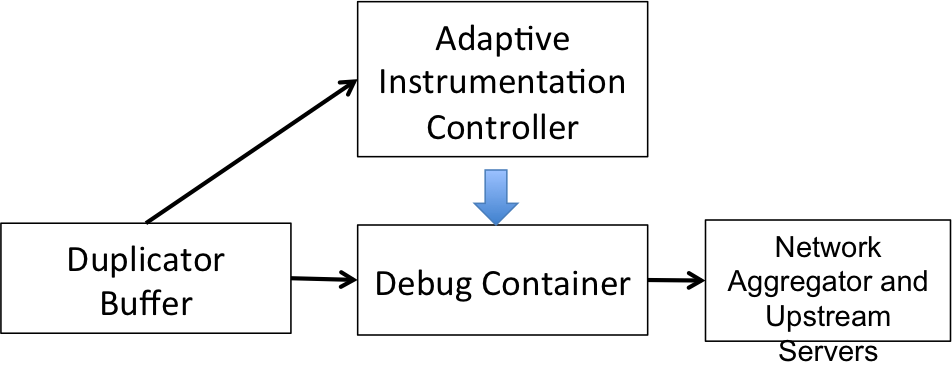
\includegraphics[width=0.96\textwidth]{queue/figs/reactive-controller.png}
		\caption{Reactive Instrumentation}
		\label{fig:reactive}
	\end{center}
\end{figure*}

A mechanism similar to TCP's network congestion avoidance mechanisms can be applied on the monitoring buffer.
We also derive inspiration from statistical debugging~\cite{statisticalPerformance,holmes,statisticalDebugging}, which shows how probabilistically instrumenting \emph{predicates}, can assist in localizing and isolating the bug. 
Predicates can be branch conditionals, loops, function calls, return instructions and if conditionals.
Predicates provide significant advantages in terms of memory/performance overheads.
Instead of printing predicates, they are usually counted, and a profile is generated.
This reduces the amount of instrumentation overhead, and several predicates can easily be encoded in a small memory space.
Similar techniques have also been applied for probabilistic call context encoding in-order to capture execution profiles with low overhead.


The sampling rate of instrumentation in the debug-container can be modified based on the amount of buffer usage.
There are three key components of our adaptive instrumentation mechanism.

\begin{itemize}
	\item \textbf{Monitoring Buffer:}
	The first step involves monitoring the buffer usage of the network duplicator. 
	If the buffer usage is more than X percentage of the buffer, the sampling rate of instrumentation can be exponentially decreased.
	This would increase the idle time in the debug container allowing it to catch up to the production and reducing the buffer usage.
	
	\item \textbf{Controller:}
	The controller allows debuggers to control the sampling rate of instrumentation.
	The sampling rate can be controlled for each predicate.
	Similar to statistical debugging the predicates with lower frequency can have higher sampling rates, and predicates with higher frequency can have lower sampling rates. This ensures overall better information gain in any profile collected.  	
	
\end{itemize}

We have looked into assigning a score to each predicate. This is based on the statistical importance of the predicate (similar to statistical debugging), and instrumentation overhead score (dependent on total budget etc.). We are still finalizing the scoring methodology.

\subsection{Feasibility}
\label{sec:queue_feasability}
\xxx{Re-label and figure out what to write here}

In ~\cite{parikshanTR,parikshanQueue} we looked into the model generation and some early theoretical experiments.
We also created a simulator in C/C++ which can buffer size, service times, overhead and incoming request rate to emulate the queuing model.
The tool shows buffer overflow, and time taken to reach the overflows.

Our initial investigation has shown that the debug container can sustain significant spikes in overhead without overflowing the production container, as long as the production container is under-capacity. 
In particular we saw a linear increase in the buffer usage for the debug-container once the workload to the production container reaches it's maximum threshold capacity.
This concurred with our earlier assumptions, as a sustained spike in the production container (such that the spike is more than the maximum threshold), would not allow the debug container to catch up.
We verified these observations both in our \parikshan prototype, as well as the simulation results shown in Appendix~\ref{appendix:simulation}.
One of the tests in our optimized linux pipe based buffer network proxy, made us realize that for smaller budgets, it is difficult to observe the increase in the buffer usage before a spike leads to an overflow.
While the simulation gives us fine grained control in our observations, our micro-evaluation on some real-world software made us realize that control in reality can be much more coarse-grained.

We are currently in the process of making an adaptive sampling instrumentation mechanism. 
For this we plan to use tools like \iprobe, systemtap~\cite{systemtap} and dyninst~\cite{dyninst}. These have been previously used in several large-scale instrumentation projects and demonstrated to be effective with low overheads. We will also derive inspiration for our model from previous statistical debugging approaches~\cite{statisticalPerformance}. These have been demonstrated to be effective in resolving several real-world bugs. This will be explored as part of the thesis.


\begin{figure}[ht]
	\centering
	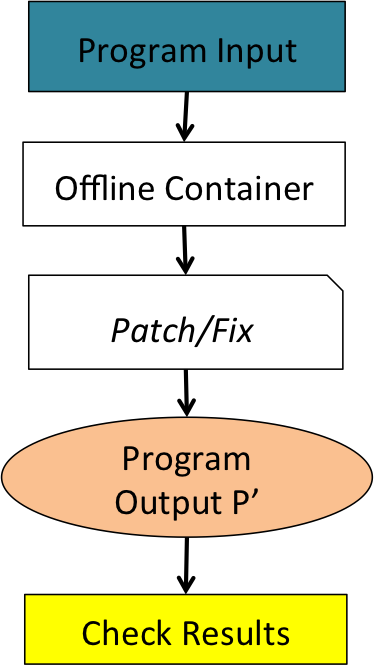
\includegraphics[width=0.25\textwidth]{guided/figs/offline.png}
	\caption{Offline Debugging}
	\label{fig:offline-debugging}
	\caption{Debugging strategies for offline debugging}
\end{figure}

\section{Active Debugging}
\label{sec:guided-approach}

In Figure~\ref{fig:offline-debugging}, we show the traditional mechanism of testing or validating patch/fixes in an application. 
In offline environments, developers apply patches and run the relevant inputs to verify that the patch works correctly. 
This is an interactive process, which allows one to verify the result and corrections before applying it to the production system.
Several cycles of this process is required, which may be followed by staged testing to ensure correctness before applying the update to the production.


\activedebugging (see figure~\ref{fig:active-debugging}) allows debuggers to apply fixes, modify binaries and apply hotpatches to applications. 
The main idea is to do a fork/exec, or parallel execution of an unmodified application.
The unmodified binary continues execution without any change in the input.
The debug-container should ideally mimic the behavior of the production, so as to allow for forward progress in the application as the debug-container will receive the same input as production.
The target process will be forked at the call of the testing function, the forked process can then be tested, the input can be transformed, or alternatively the same input can be used to validate any test-condition. 
At the end of the execution the test-process output can be checked and killed. 
The advantage of this technique is that any tests/fixes can be validated in the run-time environment itself.
This reduces the time to fix and resolve the error. 
The tests and fixes should have a local impact and should not be allowed to continue 


\begin{figure}[h]
	\centering
	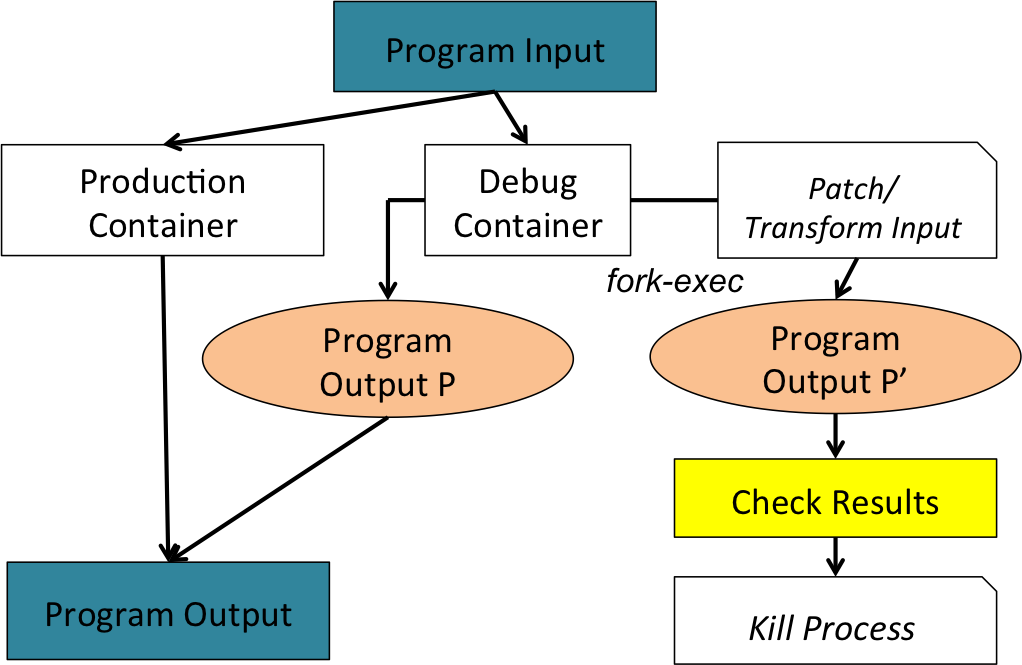
\includegraphics[width=0.75\textwidth]{guided/figs/active-debugging.png}
	\caption{Active Debugging}
	\label{fig:active-debugging}
	\caption{Debugging Strategies for Active Debugging}
\end{figure}

For Java programs, since there is no “fork”, we can utilize a JNI call to a simple native C program which executes the fork. 
Performing a fork creates a copy-on-write version of the original process, so that the process running the unit test has its own writable memory area and cannot affect the in-process memory of the original. 
Once the test is invoked, the application can continue its normal execution, while the unit test runs in the other process. 
Note that the application and the unit test run in parallel in two processes; the test does not block normal operation of the application after the fork is performed.

The fork-exec design of test-isolation ensures that the ``in-process'' memory of the process execution is effectively isolated. 
The production/debug containers are completely isolated hence the test does not impact the production in any way. 
To ensure further isolation, we propose to allow the test fork to only call wrapper libraries which allow write operations in a cloned cow filesystem.
This can be done using a COW supported filesystem with cloning functionality which are supported in ZFS and BTRFS.
For instance BTRFS provides a clone operation that atomically creates a copy-on-write snapshot of a file. By cloning the file system does not create a new link pointing to an existing inode; instead it creates a new inode that initially shares the same disk blocks with the original file. As a result cloning works only within the boundaries of the same BTRFS file system, and modifications to any of the cloned files are not visible to the original file and vice versa. 
This will ofcourse mean that we will constrain the debug/production environment to the File System of our choice.
We further propose that all test-cases in the debug-container share the test file system.


\section{Summary}
\label{sec:activeSummary}

In this chapter we presented se